\section{Datasets as a Holistic Motivating Context}

\begin{figure}
    \begin{center}
    	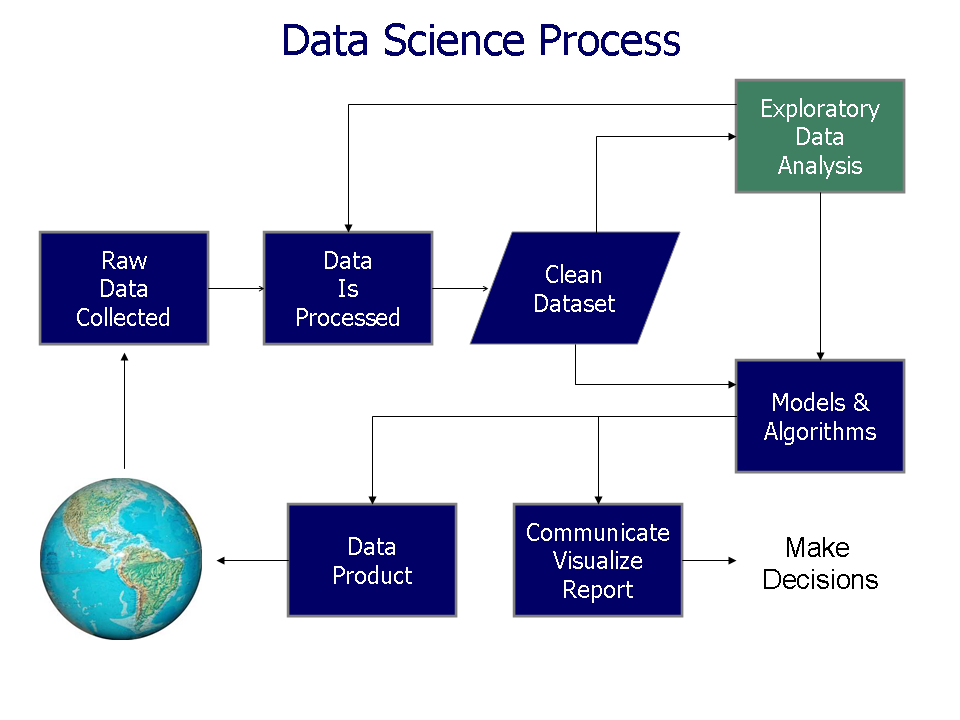
\includegraphics[width=.5\linewidth]{images/data-science.png}
    \end{center}
    \caption{A generalized model of Data Science\protect\cite{data-science-diagram}}
    \label{fig-data-science}
\end{figure}

I propose using datasets as a motivating introductory computing context.
\textbf{My core thesis is that data science, used properly, is an excellent context for motivating students across multiple components of motivation: providing opportunities for agency, a sense of usefulness and authenticity, controllable complexity, the potential to be interesting situationally and towards individualized interest, and a promotion of caring and ethics.}
Data Science accomplishes this by being a ``meta-context'' -- it is a general framework for working with an infinitely wide array of different data contexts.
However, there are many challenges in doing so -- managing data is tricky and can be a very unstructured problem.
For introductory students, in fact, it can be too overwhelming to find and dive into an arbitrary dataset, requiring significant scaffolds to get anywhere.

As established in the previous subsection, this is not a novel approach -- upper forms have always historically used datasets in courses on Machine Learning and Database Design, and recently lower forms have started too~\cite{Anderson}.
However, there is very little evaluation of the success of this approach, and numerous roadblocks exist in using this context.
For my dissertation, I will investigate what technology can be used to take full advantage of this context according to a number of constraints.
Before describing what I have done and will do, however, this section will describe this context in more detail.

\subsection{Data Science}

Data science is the process of answering questions by building, exploring, and processing datasets.
There are many theoretical models that define the term more strictly, but in general it is described as an iterative model of collecting, sanitizing, processing, rendering, and interpreting.
Figure \ref{fig-data-science} gives a visual overview of this process.
My research will not attempt to narrowly define data science; instead, the goal is simply to use elements of the data science process to contextualize the experience of learning about computing topics such as abstraction and algorithms.

It is crucial to understand that the goal is not to teach students how to become data scientists, anymore than it is the goal of Media Computation to teach students how to be professional computational artists.
As a context, using datasets is simply a means to an end -- it may involve any components of the generalized data science process at any level.
Some professors may identify data science as a learning objective in and of itself. That is fine, but they are attempting to teach something that is, at some level, distinct from computing itself.

\subsection{Big Data}

\begin{figure}
    \begin{center}
    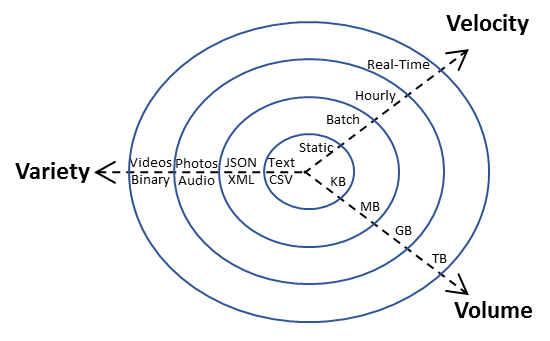
\includegraphics[width=.5\linewidth]{images/3v-model.png}
    \end{center}
    \caption{The 3V Model of Big Data}
    \label{fig-3v}
\end{figure}

One particularly important subtype of datasets is known as Big Data. Big Data is much in the news these days, from reports of massive data
dredging by the NSA to tens of millions of credit cards stolen by
hackers from commercial databases.
Big Data has become crucial to scientific advances from understanding the genome to predicting climate change.
Even more so than regular data science, there are many obstacles to effectively educating students on Big Data.
Its representation, manipulation, and expression is, by definition, challenging, and modern curriculum and programming tools are typically inadequate.

Big data has been loosely described as quantities of information that cannot be handled with traditional methods ~\cite{McKinsey}.
But ``traditional methods'' is a vague phrase that has different meanings to different learners. To a Humanities major in their first CS-0 course, the traditional method to sum a list is to use Excel. In this scenario, ``big data'' means anything that won't comfortably fit into Excel's working memory.
However, to a third-year Computer Science major, the traditional method would be to write an iterative or recursive sequential loop; being given big data forces them to explore parallel models of execution.
Clearly, ``bigness'' is a function of the learner's experience, but that is still not a solid definition.
A more precise definition is the ``3V Model'' \cite{douglas2012importance}, which posits that there are three dimensions that distinguish big data from ordinary, run-of-the-mill data:

\begin{description}
	\item[Volume:] The total quantity of the information, usually measured in bytes or number of records. However, this also extends laterally: the number of fields in the structure of the data also impacts the complexity and size. The threshold at which data becomes big is a function of the hardware and software being used. For instance, embedded systems may consider gigabyte-sized files to be big, while modern servers might not struggle until the petabyte level.
	\item[Velocity:] The rate at which new information is added to the system. High velocity big data implies a distributed architecture, since new data must be arriving from somewhere. The dynamicity of data can vary widely across these architectures, with data updating every year, every day, or even multiple times a second.
	\item[Variety:] The format or formats of the data. Ideally, data are always distributed in a way that is readily accessible. For instance, simple text-based formats such as CSV and JSON are widely supported, relatively lightweight, and human-readable. More sophisticated data formats for image and audio are also typically well-supported, although still more complicated. However, projects using specialized, compressed binary formats or, more dangerously, multiple formats (e.g., image archives organized with XML files), are more complex.
\end{description}

Silva~\cite{Silva:2014} taught an introductory course truly focused on techniques for tackling Big Data: NoSQL, MapReduce, NewSQL.
Unfortunately, they did not conduct any kind of evaluation of their work across any of the expected dimensions. 
Learning to work with Big Data can add extra authenticity to the context, but it also raises a large number of new challenges.
Once again, it is not the goal of my research to teach students how to work with truly Big datasets. Instead, I will explore whether the use of Big Data is a useful means to motivate students.